\mychapter{Introdução}
\label{cap:introducao}

Segundo \citeasnoun{ribeiro:1999}, o termo automação está relacionado com a
substituição da mão-de-obra humana ou animal por uma máquina que realize função
equivalente. Partindo desse princípio, pode-se dizer que a automação surge na
sociedade em meados do século X, com os moinhos hidráulicos que produziam
farinha. Tal mecanismo, capaz de substituir o trabalho de dez a vinte homens,
fez com que a produção de alimentos passasse por uma fase de crescimento nunca
antes observada.

Desde então, o homem tem direcionado seu conhecimento para o desenvolvimento de
tecnologias que o auxiliem em suas atividades. Com a revolução industrial, a
partir da segunda metade do século XVIII, o processo de transformação e
desenvolvimento dessas tecnologias foi acelerado, de tal forma que o homem foi
capaz de produzir uma máquina a vapor para movimentar equipamentos industriais e
de fazer um martelo de 60 quilos dar 150 golpes por minuto \cite{goeking:2010}.

Por outro lado, a utilização de sistemas de controle remete a tempos ainda mais
antigos, por volta de 300 a.C. a 250 a.C., quando foram desenvolvidas as
primeiras bóias flutuadoras, o relógio de água de Ktesíbios e uma lamparina a
óleo que matinha o nível de óleo combustível constante
\cite{mayr:1970,mayr:1971,mayr:1975}.

Já na Europa Moderna, o primeiro sistema com realimentação a ser inventado foi o
regulador de temperatura de Cornelis Drebbel, entre o final do século XVI e
início do século XVII \cite{mayr:1975}. No final do século XVII e início do
século XVIII, Dennis Papin inventou o primeiro regulador de pressão para
caldeiras a vapor. Tal dispositivo tinha funcionalidade semelhante a uma válvula
de segurança de uma panela de pressão \cite{dorf:2009}. 

% ------------------------------------------------------------------------------
\section{Aspectos históricos do controle automático}
A junção dos conceitos de automação e sistemas de controle se dá no final do
século XVIII, quando, em 1769, James Watt desenvolve o primeiro controlador
automático com realimentação usado em um processo industrial, conhecido como
{\it regulador de esferas}.

\begin{comment}
O dispositivo, inteiramente mecânico, mostrado na Fig.
\ref{fig:controlador_james}, controlava a velocidade de um motor a vapor através
do movimento de duas esferas. Na medida em que a velocidade do eixo de saída do
motor a vapor aumentava, as esferas eram elevadas (por força centrífuga) e a
válvula era fechada, diminuindo o fluxo de vapor para o motor e,
consequentemente, sua velocidade. No caso oposto, quando a velocidade de saída
do eixo do motor a vapor reduzia, as esferas eram rebaixadas, abrindo a válvula
e aumentando o fluxo de vapor para o motor, o que, consequentemente, aumentava
sua velocidade \cite{mayr:1970,mayr:1975,dorf:2009}.

\begin{figure}[htb]
\centering
    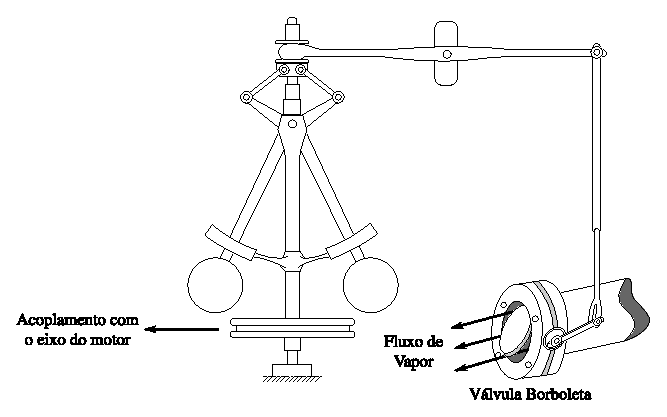
\includegraphics{imgs/introducao/eps/regulador_esferas}
    \caption{Regulador de Esferas de James Watt.}
    \label{fig:controlador_james}
\end{figure}

\end{comment}

Ainda em 1769, segundo \citeasnoun{faccin:2004}, Richard Arkwright, um inventor
inglês considerado um dos precursores das técnicas de produção em série,
acelerou o processo de industrialização ao desenvolver uma máquina de tecer
movimentada pela força da água corrente. 

Segundo o autor, foi o tear mecânico que impulsionou a Revolução Industrial na
Europa, contribuindo diretamente para a mudança dos hábitos de trabalho e das
relações sociais da Idade Contemporânea. 

De acordo com \citeasnoun{dorf:2009}, o século seguinte foi caracterizado pelo
desenvolvimento de sistemas de controle automático através da intuição e da
invenção. Esforços para aumentar a exatidão dos sistemas de controle levaram a
atenuações mais lentas das oscilações transitórias e até mesmo a sistemas
instáveis, tornando-se necessário o desenvolvimento da teoria de controle
automático.

Por volta de 1868, J. C. Maxwell formulou a teoria matemática, através das
equações diferenciais do regulador de esferas de James Watt, relacionando os
efeitos dos parâmetros do sistema com o seu desempenho \cite{maxwell:1964}. Com
o seu trabalho, Maxwell demonstrou a importância e a utilidade de modelos e
métodos matemáticos para a compreensão dos processos industriais e da teoria de
controle.

Nos anos seguintes, E. J. Routh (1877) e A. Hurwitz (1885) criaram seus
critérios de estabilidade de maneira independente
\cite{routh:1877,bennett:1996}. Mais tarde, em 1896, A. M. Lyapunov também
desenvolveu seu critério de estabilidade baseado em equações diferenciais
não-lineares de movimento \cite{faccin:2004}.

No início do século XX, por volta de 1907, foi desenvolvido o primeiro
controlador de temperatura pneumático (do tipo liga-desliga), o qual foi
instalado em uma unidade de pasteurização de leite em Nova York. Poucos anos
depois, em 1914, Edgar H. Bristol, fundador da {\it Foxboro Instrument Company},
contribuiu significativamente para o desenvolvimento de sistemas de controle ao
protocolar o pedido de patente de um amplificador denominado {\it flapper-nozzle
amplifier}, capaz de prover a ação proporcional. Em seguida, por volta de 1920,
Morris E. Leeds obteve uma patente de um controlador eletromecânico que provia a
ação integral \cite{faccin:2004}.

Em 1922, Nicholas Minorsky apresentou uma análise sobre a teoria de controle
envolvida no controle de posição, formulando a lei de controle de três termos,
hoje conhecida como controle PID.  Entretanto, até 1930 seu trabalho não havia
sido amplamente reconhecido \cite{bennett:1996}.

Somente em 1935, Ralph Clarridge criou o controlador de três termos, ao utilizar
um controlador que antecipava a variação no sinal de erro para solucionar um
problema de oscilação de uma malha de controle de temperatura em uma indústria
de celulose \cite{faccin:2004}.

% ------------------------------------------------------------------------------
\section{Introdução da automação na indústria}
Durante o período entre guerras, a teoria e a prática de sistemas de controle
nos Estados Unidos e na Europa Ocidental se desenvolveram de modo diferente do
que na Rússia e no Leste Europeu. O principal incentivo para o uso da
realimentação nos Estados Unidos foi o desenvolvimento do sistema telefônico e
dos amplificadores eletrônicos com realimentação por Bode, Nyquist e Black nos
Laboratórios Telefônicos Bell \cite{dorf:2009}.

Durante a segunda guerra mundial fez-se necessário projetar e construir pilotos
automáticos para aeronaves, sistemas de posicionamento de armas, sistemas de
controle de antenas de radares e outros sistemas militares baseados na abordagem
do controle com realimentação. A complexidade e o desempenho esperados desses
sistemas militares fizeram com que houvesse uma extensão das técnicas de
controle disponíveis além de promoverem o interesse em sistemas de controle e o
desenvolvimento de novos critérios e métodos. O projeto de sistemas de controle,
até então, era uma arte envolvendo a abordagem da tentativa e erro
\cite{dorf:2009}.

A primeira tentativa de sucesso que não levava em consideração métodos de
tentativa e erro foi proposta em \citeasnoun{ziegler:1942}. Neste artigo, foram
apresentados dois procedimentos para sintonia dos controladores através de
regras simples baseadas nas características dinâmicas do processo.

Após a disseminação dos controladores PID na industria nos anos seguintes à
publicação do artigo de Ziegler e Nichols, aconteceu o grande marco da indústria
eletrônica: a criação, em 1947, do transistor. A partir de então, começaram a
ser desenvolvidos os primeiros ``computadores industriais''. Segundo
\citeasnoun{goeking:2010}, embora o microprocessamento tenha sido comercializado
apenas a partir da década de 60, foi nesse período que surgiram os primeiros
robôs mecânicos que incorporavam os sistemas de microprocessamento e uniam
tecnologias mecânicas e elétricas.

Considerando que até o final da década de 60, as empresas automobilísticas,
apesar de produzirem em grande escala com rapidez e qualidade, não ofereciam
muitas opções de personalização para os clientes (incluindo as cores dos
acessórios), a General Motors, solicitou à empresa Allen-Bradley que
confeccionasse um produto que conferisse versatilidade à produção. A empresa que
já produzia outros dispositivos elétricos, desenvolveu em 1968, o primeiro
Controlador Lógico Programável (CLP), substituindo os antigos painéis de relés,
permitindo fazer modificações rápidas no processo produtivo \cite{goeking:2010}.

\Glossary{CLP}{Controlador Lógico Programável}

De acordo com \citeasnoun{isermann:2006}, a partir de 1975, com a
disponibilidade de microcomputadores ``baratos'', o grau de automação da
industria foi drasticamente elevado. Tal aumento ocorreu em paralelo com os
avanços dos sensores, atuadores, das redes de comunicação e das Interfaces
Humano-Computador (IHC).

\Glossary{IHC}{Interface Humano-Computador}

Desde então, a demanda cada vez mais crescente pela necessidade de maior
desempenho dos processos ou de maior qualidade dos produtos, bem como a
independência do funcionamento da planta para com os operadores humanos, vem
despertando interesse de diversos membros da comunidade científica.

%TODO citar artigos de pesquisas na área de controle/desempenho do
%processo/qualidade dos produtos

% ------------------------------------------------------------------------------
\section{A automação e supervisão de processos}
A Fig. \ref{fig:esquema_automacao} mostra um esquema simplificado da automação
de dois processos acoplados. O esquema foi dividido em três níveis: nível
inferior, o qual contempla as estratégias de controle mais comuns na industria;
nível intermediário, onde estarão os sistemas de supervisão e o nível superior,
no qual estão contidas as atividades de gerenciamento, coordenação e otimização
dos processos.

\begin{figure}[!htb]
\centering
    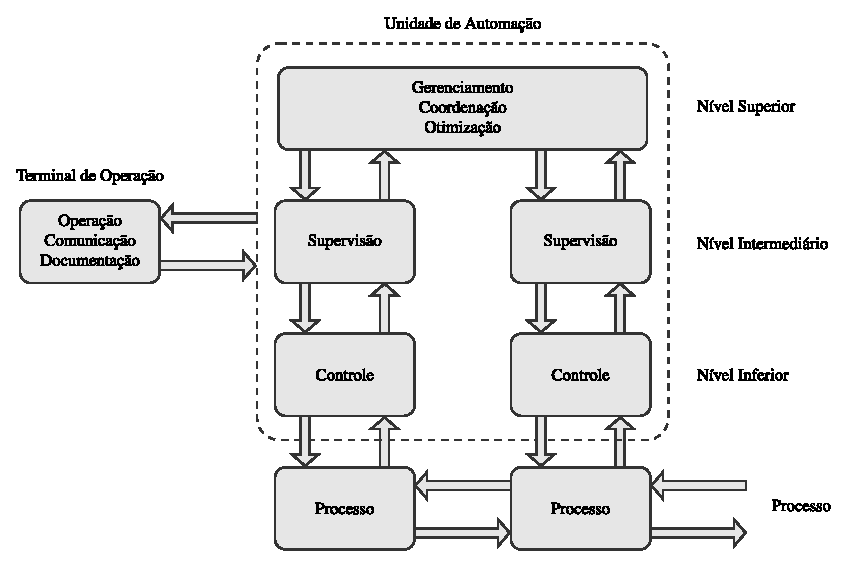
\includegraphics{imgs/introducao/eps/esquema_automacao}
    \caption{Diagrama esquemático da automação de dois processos acoplados.}
    \label{fig:esquema_automacao}
\end{figure}

Segundo com \citeasnoun{isermann:2006}, ao longo dos anos vem sendo
desenvolvendo diversos estudos sobre a teoria de controle com realimentação.
Especialmente nos sistemas de controle que incluem os observadores de estado e
estimadores de parâmetros, pode-se observar uma evolução significativa. Para o
autor, com a evolução da teoria de controle e de processamento de sinais,
diversos processos que antes possuíam um comportamento que dificultava a
elaboração de estratégias de controle, agora podem ser controlados mais
facilmente.

Entretanto, quanto mais eficiente forem as estratégias de controle no nível
inferior, melhor deverão ser as estratégias de supervisão do nível
intermediário, uma vez que os operadores são removidos do processo. Pode-se
dizer que isso ocorre porque os operadores humanos não se limitam a controlar o
processo mudando suas referências nos horários previstos, eles também realizam
a atividade de supervisão, especialmente quando estão em contato direto com o
processo. Logo, com a evolução das técnicas de controle no nível inferior, as
estratégias de supervisão também deverão ser aperfeiçoadas.

No passado, o supervisionamento automático dos processos, em sua maioria, era
composto por algum tipo de sistema que possuía a simples tarefa de verificar se
uma determinada variável, tal como {\it força}, {\it velocidade}, {\it pressão},
{\it nível} ou {\it temperatura}, ultrapassava um certo limite ou limiar
especificado para o processo. Caso isso viesse a ocorrer, um tipo de alarme
disparava, notificando o operador do ocorrido, fazendo com que este agisse de
maneira a corrigir o problema. Algumas vezes o problema podia ser corrigido
também de maneira automática por algum subsistema de proteção. Tal procedimento,
em muitos dos casos, era suficiente para evitar que houvessem falhas ou danos
graves ao processo. Por outro lado, as falhas ou os erros só eram detectados
após um certo intervalo de tempo, o que impossibilitava a obtenção de um
diagnóstico detalhado sobre o ocorrido \cite{isermann:2006}.

Os desafios desse segmento estão, portanto, em se utilizar modelos matemáticos
do processo, modelos de sinais, métodos de identificação e estimação e técnicas
de inteligência artificial para se desenvolver um sistema capaz de detectar e
diagnosticar falhas em um processo. Para se desenvolver esses tipos de sistemas,
deve-se levar em consideração diversos aspectos, destacando-se: a detecção
antecipada de pequenas falhas (abruptas ou incipientes); o diagnóstico de falhas
nos sensores, atuadores e componentes de um processo; o supervisionamento de
estados transientes; o reparo e a manutenção baseados no comportamento do
processo; o rigoroso controle de qualidade em processos de fabricação; a
detecção e diagnóstico de falhas remotas; o suporte para gerenciamento de falhas
e o suporte para sistemas tolerantes a falhas e sistemas reconfiguráveis.

Considerando tais aspectos, pode-se dizer que as primeiras publicações na área
de Detecção e Diagnóstico de Falhas (DDF) estão relacionadas com sistemas
aeroespaciais \cite{beard:1971,jones:1973,willsky:1976,clark:1978} e processos
químicos \cite{himmelblau:1978}. Os primeiros conceitos discutidos podem ser
classificados como abordagens de relação de paridade. Em tais documentos são
demonstrados procedimentos de verificação da consistência da leitura dos
instrumentos ou do balanço de massas. Outras abordagens, as quais utilizavam o
erro residual do balanço de massas foram aplicadas, por exemplo, na verificação
de vazamento em dutos \cite{billman:1987}. A abordagem de relações de paridade
foi também investigada em \citeasnoun{gertler:1985}.

\Glossary{DDF}{Detecção e Diagnóstico de Falha}

Nessa mesma época, também foram desenvolvidos métodos baseados em observadores
de estado ou filtros de Kalman \cite{beard:1971,mehra:1971,jones:1973}. Em
\citeasnoun{clark:1978}, por exemplo, um banco de observadores é utilizado para
detectar falhas em sensores através de redundância de informações. Uma variação
dos modelos de observadores de estado foi mostrada em \citeasnoun{patton:1991},
no qual se faz uso de uma estrutura de autovalores e autovetores para detecção
de falhas.

Uma outra abordagem para esse tipo de sistema fez uso de estimadores de
parâmetros, como pode ser observado em \citeasnoun{baskiotis:1979} para
aplicações com turbinas de aeronaves, em \citeasnoun{isermann:1982},
\citeasnoun{isermann:1984} e \citeasnoun{isermann:1993} para processos de
maneira geral, bombas e motores de corrente contínua, ou ainda em
\citeasnoun{filbert:1982} e \citeasnoun{filbert:1985} para aplicações envolvendo
motores elétricos.

Mais recentemente, diversas contribuições foram feitas na área de DDF. Pode-se
citar, por exemplo, as publicações relacionadas ao gerenciamento de falhas e
supervisão de processos, tais como \citeasnoun{russel:2000},
\citeasnoun{patton:2000}, \citeasnoun{higham:2001}, \citeasnoun{simani:2003},
\citeasnoun{ericson:2005}, \citeasnoun{blanke:2006}, \citeasnoun{erdenet:2007},
\citeasnoun{fesq:2009} e \citeasnoun{hang:2009}.

Em \citeasnoun{vdi2206:2003}, é mostrado um ``Diagrama em V'', que lista passos
importantes para o desenvolvimento de sistemas de DDF.
\citeasnoun{isermann:2006} diz que apesar de seguir uma sequência lógica, muitas
vezes os passos do diagrama são realizados de maneira paralela ou iterativa.

Segundo \citeasnoun{zhang:2008}, apesar das diversas pesquisas existentes desde
1970, os conceitos sistemáticos, os métodos de desenvolvimento e até mesmo as
terminologias relacionadas à área de DDF ainda não estão bem estabelecidas, o
que faz com que existam certos conflitos com a utilização correta dos termos em
cada situação específica. Algumas das contribuições sobre o assunto podem ser
observadas em \citeasnoun{laprie:1996}, \citeasnoun{avizienis:2000},
\citeasnoun{chiang:2001}, \citeasnoun{wu:2004} e \citeasnoun{isermann:2006}.

Já com relação aos métodos e algoritmos de detecção e diagnóstico de falhas,
pode-se encontrar em \citeasnoun{isermann:2006}, duas estruturas em árvore que
classificam os diversos métodos e al\-go\-rit\-mos existentes segundo
determinados critérios. Tais estruturas podem ser observadas pelas Figs.
\ref{fig:arvore_deteccao} e \ref{fig:arvore_diagnostico}.

%\begin{landscape}
\begin{figure}[htb]
\centering
    \subfigure[Métodos de Detecção]
    {
        %\includegraphics[height=0.45\textwidth]
        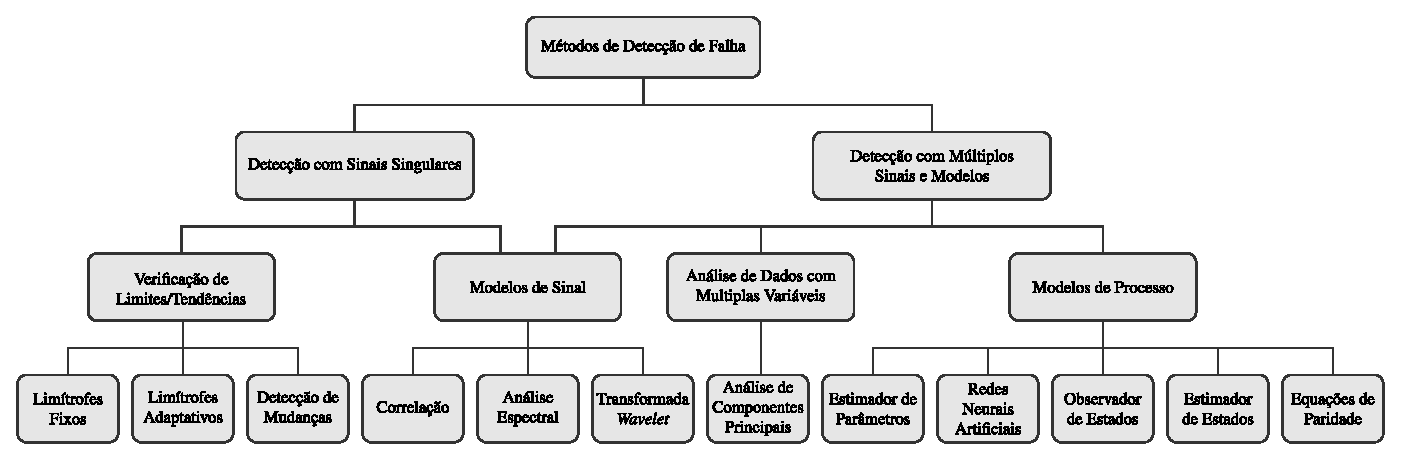
\includegraphics[width=\textwidth]
                        {imgs/introducao/eps/arvore_deteccao}
        \label{fig:arvore_deteccao}
    }
    \subfigure[Métodos de Diagnóstico]
    {
        %\includegraphics[height=0.45\textwidth]
        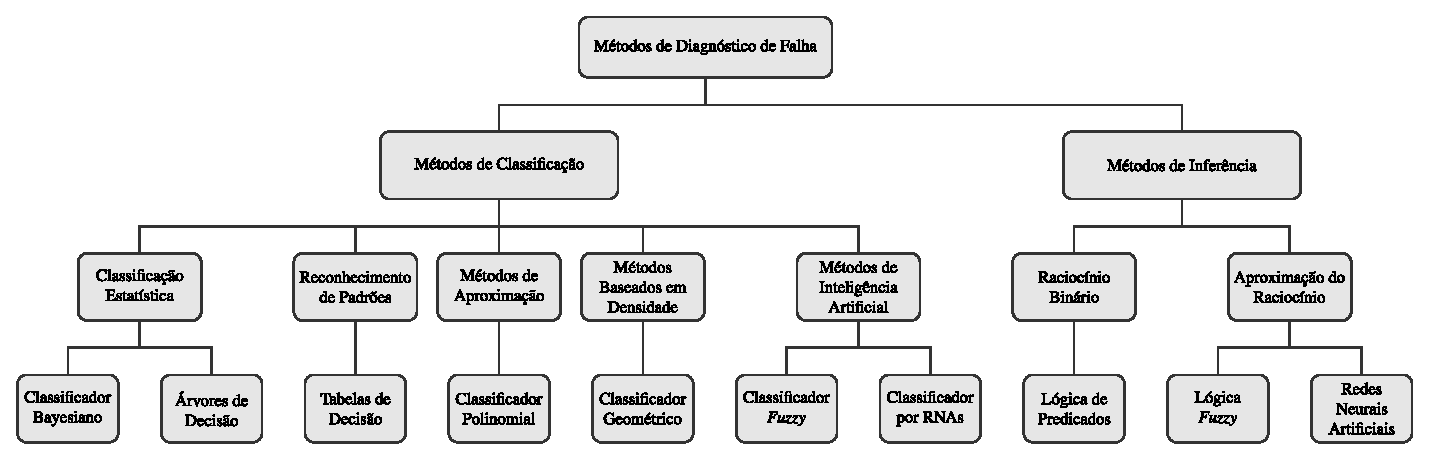
\includegraphics[width=\textwidth]
                        {imgs/introducao/eps/arvore_diagnostico}
        \label{fig:arvore_diagnostico}
    }
    \caption{Métodos de detecção e diagnóstico de falhas.}
    \label{fig:arvores_isermann}
\end{figure}
%\end{landscape}

De maneira complementar, \citeasnoun{venkatasu:2003a} subdividem os algoritmos
de diagnóstico de falhas em três classes, conforme Figs.
\ref{fig:arvore_venkatasu_quant} a \ref{fig:arvore_venkatasu_hist}. Cada uma das
classes é abordada em detalhes nos três artigos que compõem uma revisão
bibliográfica sobre o assunto
\cite{venkatasu:2003a,venkatasu:2003b,venkatasu:2003c}.

\begin{figure}[htb]
\centering
    \subfigure[Algoritmos baseados em Análise Quantitativa]
    {
        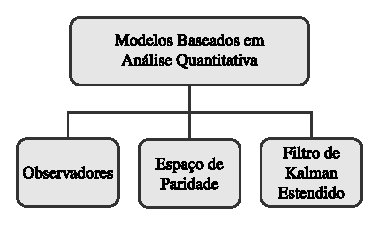
\includegraphics[width=0.3\textwidth]
                        {imgs/introducao/eps/arvore_venkatasu_quant}
        \label{fig:arvore_venkatasu_quant}
    }
    \qquad
    \subfigure[Algoritmos baseados em Análise Qualitativa]
    {
        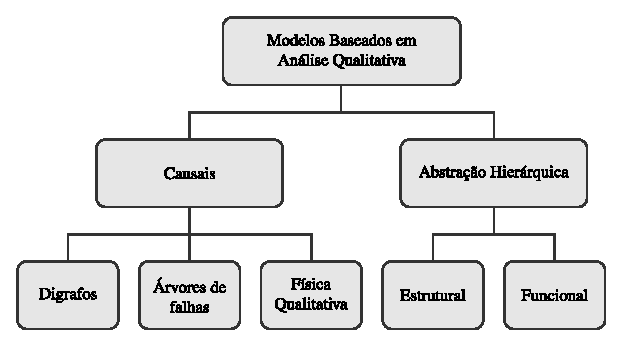
\includegraphics[width=0.51\textwidth]
                        {imgs/introducao/eps/arvore_venkatasu_qual}
    }
    \subfigure[Algoritmos baseados em Histórico do Processo]
    {
        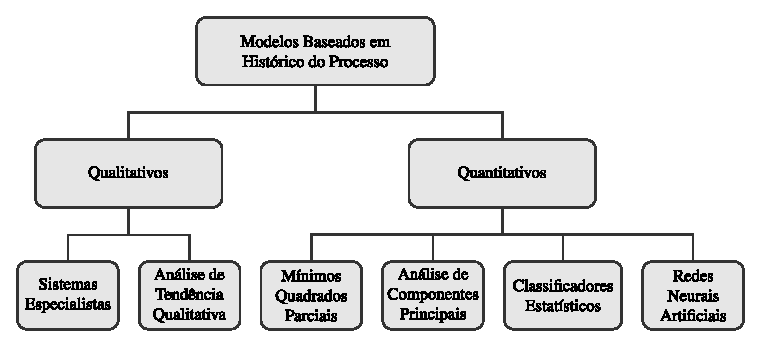
\includegraphics[width=0.6\textwidth]
                        {imgs/introducao/eps/arvore_venkatasu_hist}
        \label{fig:arvore_venkatasu_hist}
    }
    \caption{Classificação dos algoritmos de diagnóstico de falhas.}
    \label{fig:arvore_venkatasu}
\end{figure}

\begin{comment}
\citeasnoun{zhang:2008} tratam ainda sobre diversos tópicos relacionados aos
Sistemas de Controle Tolerante a Falhas (SCTF), outro segmento de pesquisa até
então não mencionado. Mostram para isso que, por razões históricas e por
questões de complexidade, a maioria das pesquisas relacionadas à DDF e às
estratégias de controle reconfiguráveis foram realizadas como duas coisas
separadas. Afirmam também que pouca atenção é dada para a construção de um
sistema ``completo'' que possua essa interação entre um sistema de detecção e
diagnóstico e as estratégias de controle reconfiguráveis.

\Glossary{SCTF}{Sistema de Controle Tolerante à Falhas}

Sendo mais específico, os autores mostram que as técnicas de detecção e
isolamento de falhas foram desenvolvidas como ferramentas de diagnóstico ou de
monitoramento. Como resultado disso, aduzem que os métodos de detecção e
diagnóstico não satisfazem as necessidades das técnicas de controle
reconfigurável, em contraste com o que é exposto na maioria das pesquisas na
área de controle reconfigurável, nas quais assume-se a existência de um sistema
de detecção e diagnóstico perfeito.
\end{comment}

Tendo conhecido alguns dos temas mais abordados ao longo de todos esses anos, o
trabalho a ser aqui apresentado se propõe a desenvolver um sistema que faça uso
de Redes Neurais Artificiais (RNAs) para detectar e diagnosticar as falhas que
venham a ocorrer em um determinado processo dinâmico. O sistema deverá ser capaz
de detectar a presença das falhas, gerando sinais de alarme que notifiquem o
operador e que possam vir a ser pós-processados.

\Glossary{RNA}{Rede Neural Artificial}

Para que isso seja possível, o modelo de estudo de caso será identificado
através de redes neurais, de tal modo que a partir do valor real mensurado e da
inferência realizada pelo modelo identificado, seja gerado um resíduo que, em
conjunto com outros valores, irão compor a entrada da estrutura neural de
detecção e diagnóstico de falhas.

Considerando então os métodos de DDF que fazem uso de RNAs, pode-se destacar uma
série de contribuições. Em \citeasnoun{sreedhar:1995}, por exemplo, é elaborado
um sistema que possui uma rede neural adaptativa capaz de detectar falhas em
sistemas não-lineares. \citeasnoun{vemuri:1998}, por sua vez, propõe um sistema
de detecção de falhas inteligente para manipuladores robóticos. Já em
\citeasnoun{chang:2003} é desenvolvido um sistema que faz uso de RNAs para
detectar curto-circuitos. Em \citeasnoun{talebi:2005} é mostrada uma estrutura
capaz de detectar falhas em sistemas de controle de satélites.
\citeasnoun{jia-li:2010} mostra ainda um sistema capaz de diagnosticar falhas em
sistemas de câmbio automotivo.

Diversas outras contribuições foram feitas através da utilização de técnicas
híbridas. Em \citeasnoun{gao:2000}, por exemplo, é proposto um sistema que
utiliza uma rede neural de Elman, com treinamento assistido por algoritmo
genético para a detecção de falhas em unidades de sistemas de motor.
\citeasnoun{guo:2005} combinam as propriedades das transformadas {\it wavelet}
com RNAs para detecção de falhas em máquinas rotativas Já em
\citeasnoun{tian:2007}, é proposto um sistema Neuro-{\it Fuzzy} para detecção de
falhas em oleodutos. Por fim, \citeasnoun{khaled:2010}, mostra um sistema
composto por um método que combina RNAs com análise de componentes principais,
capaz de identificar e isolar falhas em processos de fabricação.

Assim sendo, os capítulos seguintes do presente texto serão divididos conforme
descrição a seguir. O Capítulo \ref{cap:rnas} irá abordar os conceitos sobre as
RNAs, mostrando suas arquiteturas e modelos de identificação que serão
utilizados no trabalho. Em seguida, o Capítulo \ref{cap:detec_diag} irá tratar
sobre as terminologias utilizadas e os métodos de detecção e diagnóstico de
falhas. Já o Capítulo \ref{cap:sistema}, irá conter a descrição detalhada do
processo escolhido como estudo de caso e mostrará algumas possibilidades de como
o sistema final poderá ser composto. Por fim, nos dois últimos capítulos, serão
apresentados e discutidos os resultados obtidos para cada uma das estruturas
idealizadas no Capítulo \ref{cap:sistema}, encerrando com uma breve conclusão e
mostrando as possibilidades de trabalhos futuros.
